\chapter{Implementation}
\label{chap:impl}


preliminary structure:

1. architecture
2. technical details (memory included)
3. modules details


overview of architecture (.exm -> lexer -> parser -> compiler (code gen) -> .yul code -> solidity compiler -> EVM bytecode)
                                                           |
                                                           -> ABI generator

detailed overview of modules (for example: calldata parsing, compiler (two passes), return data transformer, storage)


technical details:
  - memory organization
    - how variables are stored, dynamic typing
    - immutability of variables
    - offset
  - show events/module args syntax
  - key features
    - events
    - constructor
    - storage
    - ABI for public functions
    - reverts with utf-8 error string
  - standard functions declaration on demand (transitivity included) and mechanism itself (module responsible for )

\section{Architecture overview}
\label{sec:architecture}

This section outlines the principal elements of the design of Elixireum compiler. It overviews the technology stack employed in the development process and underscores the pivotal decisions that shaped the architecture of the compiler.


\subsection{Choice of Elixir}
Here is the racialization behind the choice of Elixir:
\begin{itemize}
    \item The most popular open source Web3 explorer, Blockscout\footnote{\href{https://www.blockscout.com/}{Official Blockscout website}}, is written in Elixir. From this we can say that Elixir is well heard of in Web3 community.
    \item Our team possesses substantial expertise in this programming language.
    \item Elixir is open source so we can easily reuse its machinery for tokenization and parsing Elixireum.
\end{itemize}

\subsection{Choice of Yul}
\begin{itemize}
    \item Initially, our strategy entailed compiling Elixireum directly into Ethereum Virtual Machine (EVM) bytecode. Subsequently, we pivoted towards an intermediate representation (IR), selecting Yul as IR aligned with our requirements. Advantages from this decision encompass:
        \begin{itemize}
            \item Compatibility with all EVM versions, obviating the need for version-specific concerns.
            \item Avoidance of reimplementing primitives such as function calls, variable and stack management, thereby freeing up resources to enhance the feature set of the language.
            \item Reduced gas consumption facilitated by the ability to optimize Yul code of Solidity compiler.
        \end{itemize}
    \item Despite these considerations, the choice comes with limitations, notably:
        \begin{itemize}
            \item Dependency on the Solidity compiler for Elixireum.
        \end{itemize}

        No significant downsides compared to direct compilation to EVM bytecode, as bytecode can be used in Yul directly.
    \item We considered the mapping of BEAM (Erlang VM) bytecode to EVM bytecode as an option as well. This option was deemed challenging due to the fundamental architectural and philosophical differences between the two virtual machines. BEAM is specifically tailored for environments that demand high concurrency, distribution, and fault tolerance, boasting a set of opcodes optimized for these conditions. In contrast, the EVM is built to run smart contracts within blockchain ecosystems, prioritizing deterministic execution and gas metering to safeguard against spam and enhance the security of the network. Due to these distinct focuses, BEAM incorporates specialized instructions for concurrency and distributed processing, which do not directly translate to EVM.
\end{itemize}


\begin{figure}[h!]
    \centering
    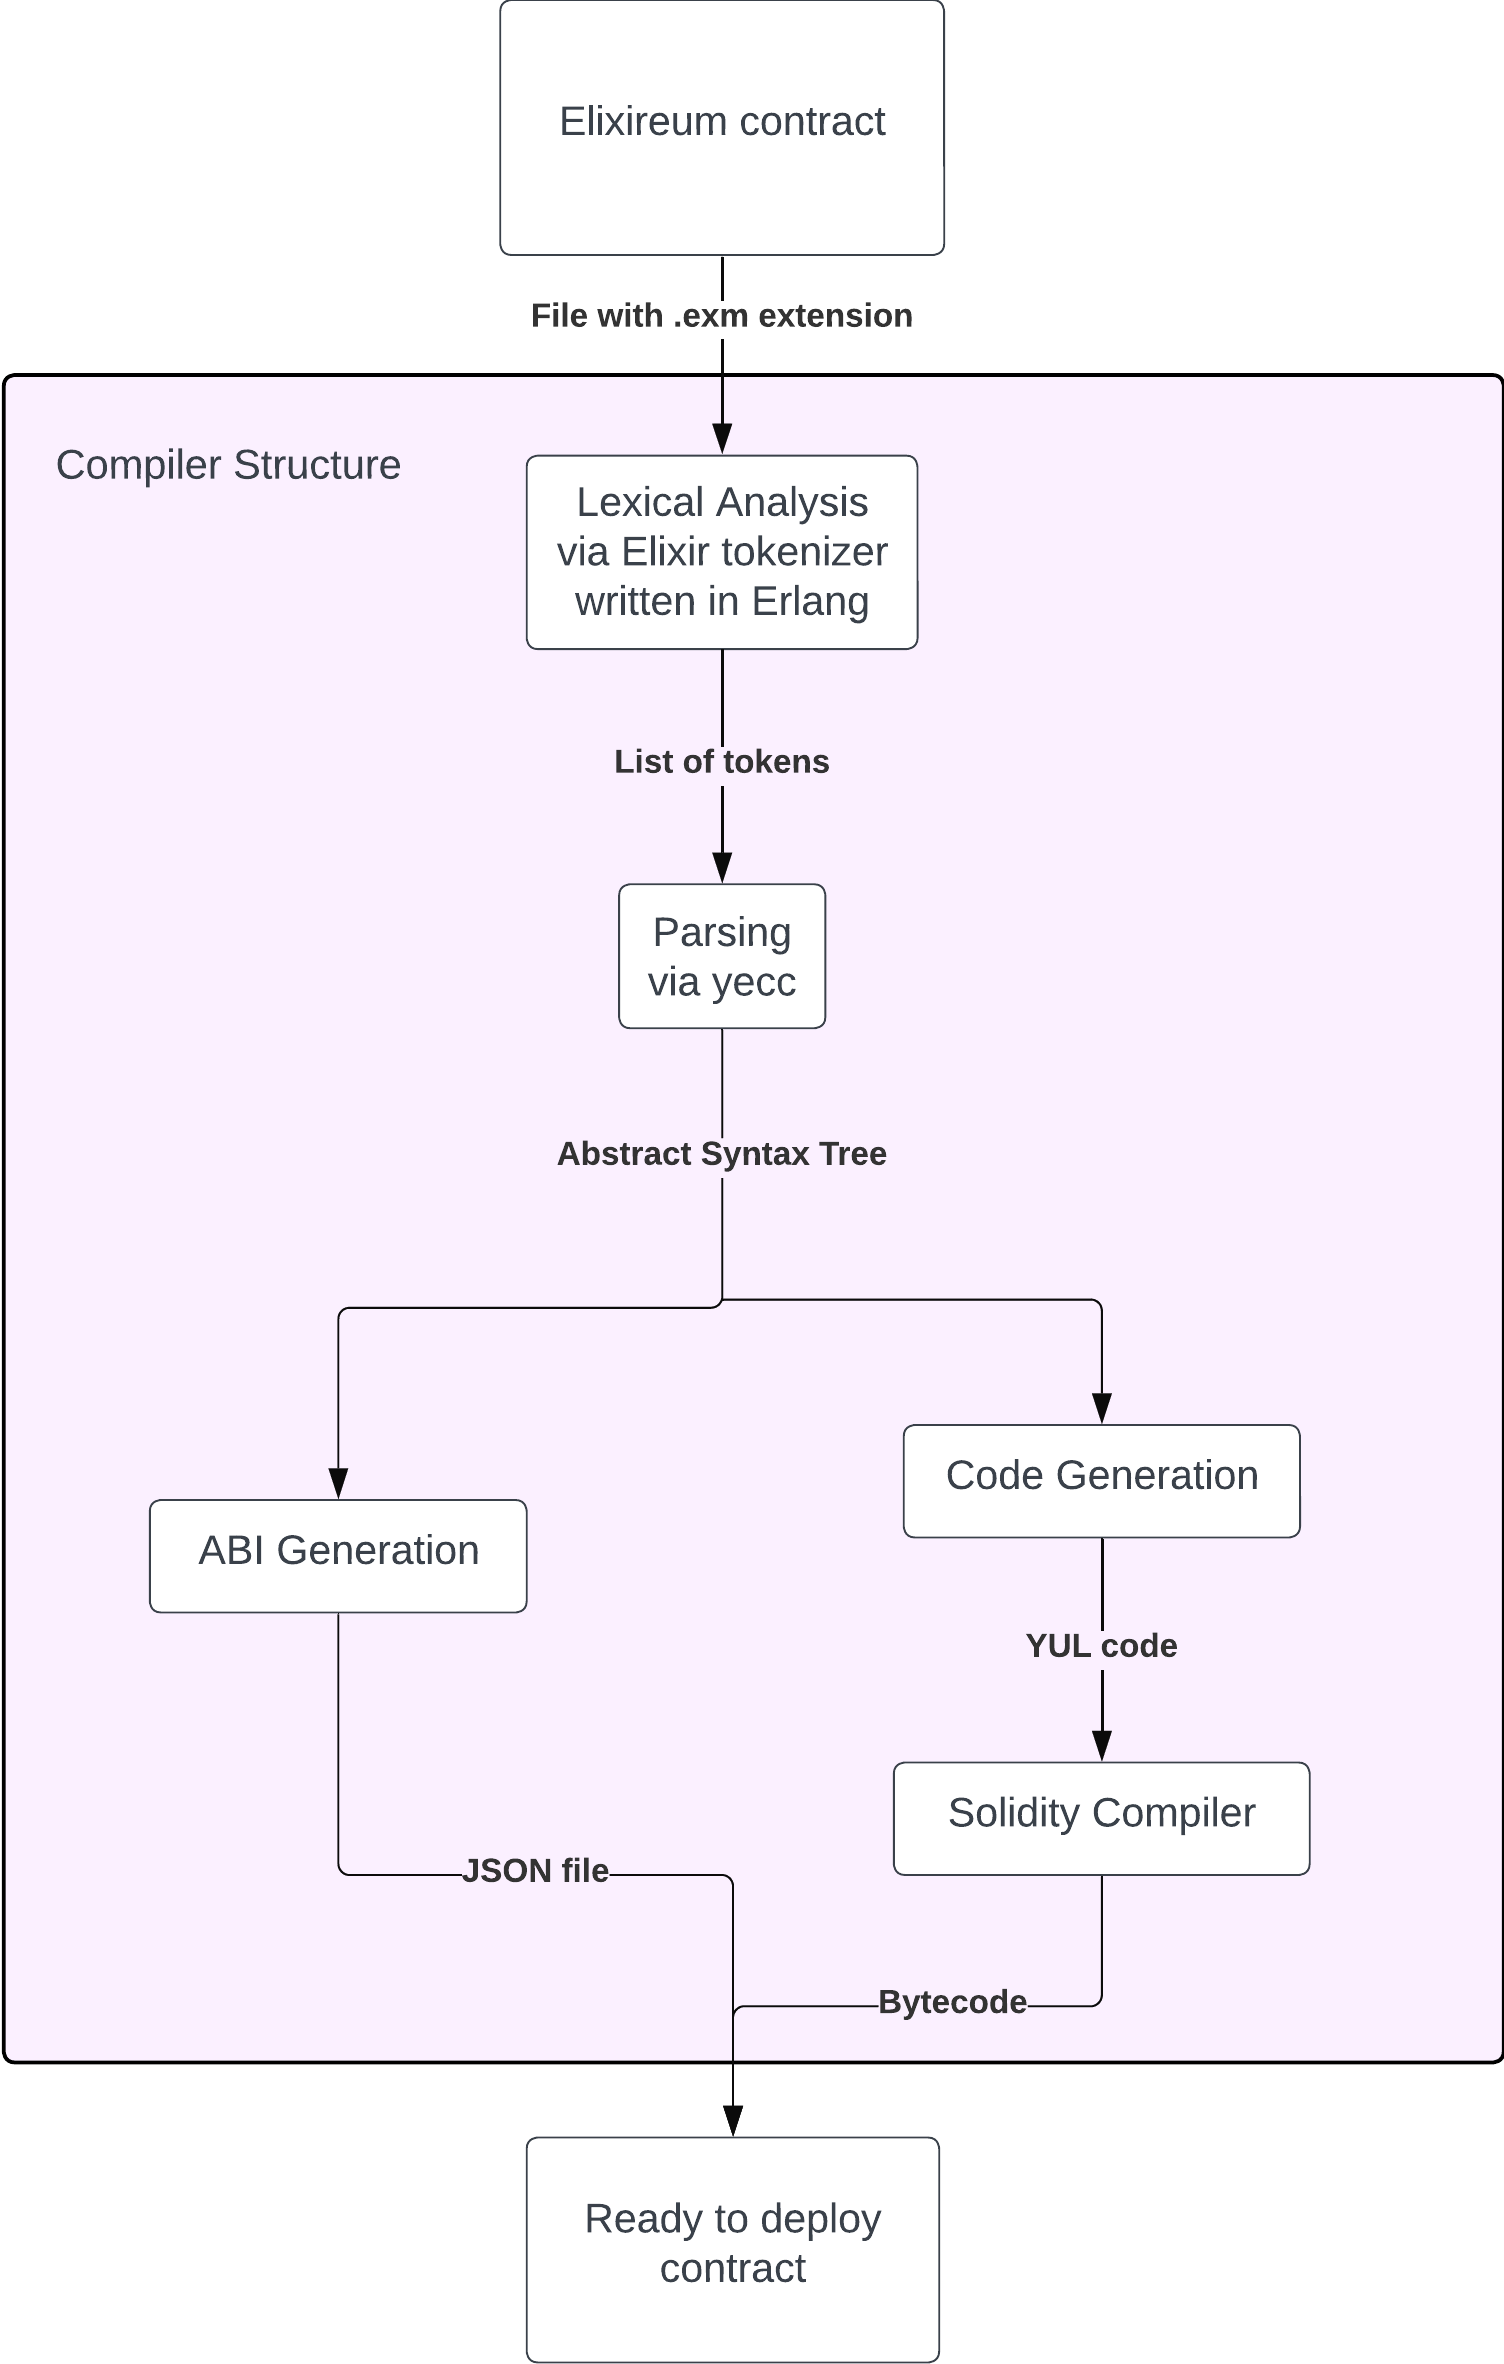
\includegraphics[width=0.8\textwidth]{figs/arch.png}
    \caption{Elixireum compiler architecture}
    \label{fig:arch}
\end{figure}

\section{Technical details}

\subsection{Memory organization}
\label{sec:memory_organization}

In implementation of our language we decided to store all the runtime variables in volatile memory of EVM. The choice is rationalized by a small gas cost of memory operating and the easiness of implementation. There was two alternates: transient storage (cost more than memory) and stack (more complex management). Each new variable is stored after the previous
In generated yul code variable is defined as pointer to a memory where the value is located. At this pointer first byte is reserved for the type number. The next X bytes is the value itself (for simple cases). For the complex cases like lists, tuples: first byte as for primitives is the type, the next word\footnote{in this context word is 32 bytes} is the count of elements, then the elements itself, one by one. Each element is inplace variable (type + value). For strings or bytes: 1st byte -- type (1 -- string, 102 -- bytes), next word -- bytes count (X), then all X bytes one by one.

Example for simple case:
   
\begin{lstlisting}[caption={Elixireum code for simple case}, language=elixir]
  a = 1
  b = 2
\end{lstlisting}

\begin{lstlisting}[caption={Generated yul code for simple case}, language=yul]
  let offset$ := msize()      // define offset$, set it to current memory size 
  let a$ := offset$           // define variable as the memory pointer
  mstore8(offset$, 67)        // 67 is int256 type
  offset$ := add(offset$, 1)  // increase current offset by 1 byte, which is used by type on the line above
  mstore(offset$, 1)          // store the value itself
  offset$ := add(offset$, 32) // int256 value takes 32 bytes

  let b$ := offset$           // define variable as the memory pointer
  mstore8(offset$, 67)        // 67 is uin256 type
  offset$ := add(offset$, 1)  // increase current offset by 1 byte, which is used by type on the line above
  mstore(offset$, 2)          // store the value itself
  offset$ := add(offset$, 32) // int256 value takes 32 bytes
\end{lstlisting}

\begin{table}[h!]
  \centering
  \renewcommand{\arraystretch}{1.2} % Reduces the height of the table
  \begin{tabular}{|>{\centering\arraybackslash}m{2cm}|>{\centering\arraybackslash}m{1cm}|>{\centering\arraybackslash}m{1cm}|>{\centering\arraybackslash}m{1cm}|>{\centering\arraybackslash}m{0.75cm}|>{\centering\arraybackslash}m{1cm}|>{\centering\arraybackslash}m{1cm}|>{\centering\arraybackslash}m{1cm}|>{\centering\arraybackslash}m{1cm}|>{\centering\arraybackslash}m{0.75cm}|>{\centering\arraybackslash}m{1cm}|}
  \hline
  \textbf{Addresses} & 0x00 & 0x01 & 0x02 & ... & 0x21 & 0x22 & 0x23 & 0x24 & ... & 0x42 \\ \hline
  \textbf{Values}    & 0x43 & 0x00 & 0x00 & ... & 0x01 & 0x43 & 0x00 & 0x00 & ... & 0x01 \\ \hline
  \end{tabular}
  \caption{EVM Memory snippet for simple case}
  \label{tab:evm_memory}
  \end{table}

Example for string

\begin{lstlisting}[caption={Elixireum code for string case}, language=elixir]
  a = "abc" # hex representation of this utf-8 string is 0x616263
\end{lstlisting}
  
\begin{lstlisting}[caption={Generated yul code for string case}, language=yul]
  let offset$ := msize()      // define offset$, set it to current memory size 
  let a$ := offset$           // define variable as the memory pointer
  mstore8(offset$, 1)         // store the type, 1 is the string type
  offset$ := add(offset$, 1)  // increase current offset by 1 byte, which is used by type on the line above
  mstore(offset$, 3)          // store the byte size of the string
  offset$ := add(offset$, 32) // increase current memory pointer by 32 bytes, since the size of the string is 256 bit lenght
  mstore(offset$, 0x6162630000000000000000000000000000000000000000000000000000000000) \\ store the string itself
  offset$ := add(offset$, 3)  // string has length only 3 bytes
\end{lstlisting}
  
\begin{table}[h!]
  \centering
  \renewcommand{\arraystretch}{1.2} % Reduces the height of the table
  \begin{tabular}{|>{\centering\arraybackslash}m{2cm}|>{\centering\arraybackslash}m{1cm}|>{\centering\arraybackslash}m{1cm}|>{\centering\arraybackslash}m{1cm}|>{\centering\arraybackslash}m{0.75cm}|>{\centering\arraybackslash}m{1cm}|>{\centering\arraybackslash}m{1cm}|>{\centering\arraybackslash}m{1cm}|>{\centering\arraybackslash}m{1cm}|}
  \hline
  \textbf{Addresses} & 0x00 & 0x01 & 0x02 & ... & 0x20 & 0x21 & 0x22 & 0x23 \\ \hline
  \textbf{Values}    & 0x01 & 0x00 & 0x00 & ... & 0x03 & 0x61 & 0x62 & 0x63 \\ \hline
  \end{tabular}
  \caption{EVM Memory Organization}
  \label{tab:evm_memory}
  \end{table}

Example for list:

\begin{lstlisting}[caption={Elixireum code for list case}, language=elixir]
  a = [1, true, "abc"]
\end{lstlisting}
  
\begin{lstlisting}[caption={Generated yul code for string case}, language=yul]
  let offset$ := msize()
  
  let var0$ := offset$
  mstore8(offset$, 67)
  offset$ := add(offset$, 1)
  mstore(offset$, shl(0, 1))
  offset$ := add(offset$, 32)
  
  let bool_var1$ := offset$
  mstore8(offset$, 2)
  offset$ := add(offset$, 1)
  mstore8(offset$, true)
  offset$ := add(offset$, 1)

  let str2$ := offset$
  mstore8(offset$, 1)
  offset$ := add(offset$, 1)
  mstore(offset$, 3)
  offset$ := add(offset$, 32)
  mstore(offset$, 0x6162630000000000000000000000000000000000000000000000000000000000)
  offset$ := add(offset$, 3)

  let list3$ := offset$
  mstore8(offset$, 103)
  offset$ := add(offset$, 1)
  mstore(offset$, 3)
  offset$ := add(offset$, 32)
  let ignored_
  ignored_, offset$ := copy_from_pointer_to$(var0$, offset$)
  ignored_, offset$ := copy_from_pointer_to$(bool_var1$, offset$)
  ignored_, offset$ := copy_from_pointer_to$(str2$, offset$)



  let $_a := list3$



  
  let offset$ := msize()      // define offset$, set it to current memory size 
  let a$ := offset$           // define variable as the memory pointer
  mstore8(offset$, 1)         // store the type, 1 is the string type
  offset$ := add(offset$, 1)  // increase current offset by 1 byte, which is used by type on the line above
  mstore(offset$, 3)          // store the byte size of the string
  offset$ := add(offset$, 32) // increase current memory pointer by 32 bytes, since the size of the string is 256 bit lenght
  mstore(offset$, 0x6162630000000000000000000000000000000000000000000000000000000000) \\ store the string itself
  offset$ := add(offset$, 3)  // string has length only 3 bytes
\end{lstlisting}
  
\begin{table}[h!]
  \centering
  \renewcommand{\arraystretch}{1.2} % Reduces the height of the table
  \begin{tabular}{|>{\centering\arraybackslash}m{2cm}|>{\centering\arraybackslash}m{1cm}|>{\centering\arraybackslash}m{1cm}|>{\centering\arraybackslash}m{1cm}|>{\centering\arraybackslash}m{0.75cm}|>{\centering\arraybackslash}m{1cm}|>{\centering\arraybackslash}m{1cm}|>{\centering\arraybackslash}m{1cm}|>{\centering\arraybackslash}m{1cm}|}
  \hline
  \textbf{Addresses} & 0x00 & 0x01 & 0x02 & ... & 0x20 & 0x21 & 0x22 & 0x23 \\ \hline
  \textbf{Values}    & 0x01 & 0x00 & 0x00 & ... & 0x03 & 0x61 & 0x62 & 0x63 \\ \hline
  \end{tabular}
  \caption{EVM Memory Organization}
  \label{tab:evm_memory}
  \end{table}

yul:

Example of an array:
exm:
  a = [1, true, "a"]
runtime EVM memory:
  0x0

Since we developed a functional language one of the fundamental principle of which is immutability, each assignment operation is a creation of new variable, i.e. we "forget" previous pointer, assign new pointer and put the variable to the new place.

Each new variable should be placed after the previous, for this purpose we define in the generated yul code the variable offset\$. This variable tracks the last allocated memory address + 1. As the workaround for corner cases we update this variable via msize() call, assigning to the offset\$ variable current memory size rounded to 1 word.


\section{Modules overview}
This section provides detailed overview of main modules of the compiler. Modules are listed in the order corresponding to contract life cycle, i.e. deployment then calls.
\subsection{Compiler}
Here is the pipeline of actions performed by the main Compiler module, the error on any step is thrown  
\begin{itemize}
    \item Reading source code from the file system.
    \item Run Elixir tokenizer and parser on the source code.
    \item Perform the first pass of Elixir AST in pre-order to gather information about defined functions, storage variables and events. At this step compiler checks that public defined functions have corresponding typespecs, storage variables have type and events have all required fields.
    \item Perform the second pass of Elixir AST in post-order to generate Yul code. Specifically, the compiler generates so called function selector, function selector is used to identify which function is being called based on the first four bytes of call data. First four bytes of the calldata are four bytes of Keccak256 of the string of the following format function_name \lef type_of_the_first_argument,type_of_the_second_argument,\dots)
    % \texttt{function_name()}
    % , this is called method id. For example if the function has the following signature deposit\(address depositAsset, uint256 depositAmount, uint256 minimumMint\), the Keccak256 is performed on deposit\(address,uint256,uint256\)
    
    , it is 0x0efe6a8b11bdbb92d49045fffbd9e8dc4b5b43f7a0459dae9c8fdf27311f275e, the first four bytes of this hash is the method id of deposit function. Function selector is simply the switch case expression where each public definid function corresponds to case with its method id. In the cases function arguments decoding from calldata generated using the calldata decoding module, then function call generated as if it was a private function, then compiler generated the code that encodes the value returned by the function to return format using the return data encoding module. Then, compiler generates Yul code for all user defined functions, both public and private, as difference between public and private function is factored out to function selector. 


\end{itemize}
\subsection{ABI generator}
\subsection{Calldata decoding}
\subsection{Emitting events}
\subsection{Return data encoding}


% \begin{longtable}{c|c}
% \caption[This is the title I want to appear in the List of Tables]{Simulation Parameters} \label{table:fousimulation_params} \\
% \hline
% A & B  \\
% \hline
% \endfirsthead
% \multicolumn{2}{@{}l}{} \\
% \hline
% A & B \\
% \hline
% \endhead
% \hline
%  \textbf{Parameter} & \textbf{Value}\\
%  \hline
%  Number of vehicles & $|\mathcal{V}|$\\
%  \hline
%  Number of RSUs & $|\mathcal{U}|$\\
%  \hline
%  RSU coverage radius & 150 m\\
%  \hline
%  V2V communication radius & 30 m\\
%  \hline
%  Smart vehicle antenna height & 1.5 m\\
%  \hline
%  RSU antenna height & 25 m\\
%  \hline
%  Smart vehicle maximum speed & $v_{max}$ m/s\\
%  \hline
%  Smart vehicle minimum speed & $v_{min}$ m/s\\
%  \hline
%  Common smart vehicle cache capacities & $[50, 100, 150, 200, 250]$ mb\\
%  \hline
%  Common RSU cache capacities & $[5000,1000,1500,2000,2500]$ mb\\
%  \hline
%  Common backhaul rates & $[75, 100, 150]$ mb/s\\
%  \hline
% \end{longtable}

% \begin{figure}[hbt]
% \centering
% 
\includegraphics[]{figs/inno.png}
% \caption{One kernel at $x_s$ (\emph{dotted kernel}) or two kernels at
% $x_i$ and $x_j$ (\textit{left and right}) lead to the same summed estimate
% at $x_s$. This shows a figure consisting of different types of
% lines. Elements of the figure described in the caption should be set in
% italics, in parentheses, as shown in this sample caption.}
% \label{fig:fouex}
% \end{figure}

% \ldots
